\section{First Principles}
\label{sec:org6a628ce}
The three parts of this thesis each had a slightly different focus, spanning the range of methodologies which is characteristic for biomechanical research (kinematics, dynamics, statistics).
They follow a common scheme:
each of the parts took a basic principle of physics research and applied it to the study of biomechanics.


Part one was concerned with kinematic data analysis, and the generation of meaningful measures from videos of moving animals.
The basic principle therein is coordinate transformation \citep{Tipler2007}: physicists are well aware that computational problems simplify if one converts the data to an appropriate coordinate space.
For locomotor kinematics, I reproduced and applied a suggestion of others \citep{Bernstein1927a,Webb2007} which relies on the repetitive, periodic character of many locomotor behaviors (Ch. \ref{cpt:fourier_review}).
By applying a Fourier Series Decomposition, it is possible to transform joint angle profiles to the frequency domain, where their mathematical structure is much simplified (affine components are accessible; time series are represented by an array of harmonic constituents, instead of a raw signal with an undefined number of noisy samples).
The Fourier Series method is a flexible tool which opens up a data set to multivariate statistics (Ch. \ref{cpt:fcas}).
It is also a prerequisite of the subsequent part, which could hardly be adapted to untransformed kinematic measures.

\medskip
Part two focused on statistical modeling of kinematic measurements.
It built on the application of another physical principle: namely that most measured variables do not take exact values, but rather follow probability distributions \citep{2022Probability}.
This is especially true in the biological sciences, where variability in a trait, in reproductive success, and in the correlation of these two are the key prerequisites of our central working model \citep{Darwin1859}.
Statistical models which incorporate variability, though rarely applied in that context to date, are useful in biological applications \citep{Roraas2019,DeGroote2021}.
I provided a brief tutorial to outline why and how probabilistic models work in practice (e.g. the MCMC sampling methodology, Ch. \ref{cpt:statistics}).
In that framework, I applied probabilistic, predictive modeling to a comprehensive data set of piglet kinematics (Ch. \ref{cpt:piglets}).
Prediction in conventional statistics would be deterministic, i.e. yielding \chng{averages, at best with the vague guidance of standard deviations,} which only superficially capture the stochastic, variable nature of the phenomenon.
I demonstrated that probabilistic prediction can be used to generate relevant insights into locomotor maturation of piglets.

\medskip
Finally, the third part of the thesis was devoted to inverse dynamics.
The goal of inverse dynamics are estimates of joint forces and moments, which can be calculated from measured or estimated external forces and moments by treating limb segments as rigid bodies, and by (stepwise) calculation of their balance of wrenches (Ch. \ref{cpt:dynamics_workflow}).
Rigid bodies must be associated with inertial properties (mass, center of mass, mass moment of inertia), which are crucial prerequisites for the balance equations.
As I then demonstrated, the assumption that inertial properties can be accurately derived from x-ray computed tomography cannot stand up to closer inspection (Ch. \ref{cpt:inertials}).
They can be derived, but not accurately, yet they might provide the ``best educated guess'' available.
This finding was enabled by a third basic principle commonly applied in physics (which is actually a first principle): the quantification of a measurements inaccuracy \citep{Hughes2010}.

\medskip
There are certainly more examples of basic principles in physics which would deserve application in biology in general \citep[e.g. quantum cognition,][]{Busemeyer2015,Aerts1995}, or in biomechanics in particular \citep[e.g. wrenches and quaternions,][]{Dumas2004}.
\section{\chng{Predictive Power}}
\label{sec:org9f5e4a8}
Yet are these adaptations from the physical sciences inevitable?
Why/when should conventional methods be questioned and compared to the yet uncommon methods suggested in this thesis?


The two decisive analysis characteristics are the occurrence of variability, and predictive modeling.

Variability is omnipresent in biology, and I find it surprising how many studies use statistics which model point estimates for actually variable measurements.

Yet the ultimate quality criterion of statistical models (and classifiers, and neural networks/``AI'') is how well they can be used to predict experimental circumstances which deviate from those they were trained on, or in other words how they transfer to novel circumstances.
This refers to the distinction of descriptive, explanatory, and predictive modeling \citep{Shmueli2010,Shmueli2011}.
In biomechanics, explanatory modeling is rarely applied, because the cause for animal movement are known to be physical first principles (conservation of momentum, Ch. \ref{cpt:dynamics_workflow}).
Virtually all quantitative analyses in locomotor science are descriptive: they ``summarize or represent the data structure in a compact manner'', and ``focus is at the measurable level rather than at the construct level'' \citep{Shmueli2010}.
For example, spatiotemporal gait characteristics (e.g. dimensionless speed) are often measured and compared between study groups.
There are numerous recent examples of studies in which spatiotemporal gait variables are the basis and (own) goal of comparison  \citep[e.g.][]{Cheu2022,Ekhator2023,Plocek2023,Young2023,Jones2023,Druelle2021,McHenry2023}.
However, it is rarely modeled how and why a study group reaches a certain speed (explanatory statistics), and the predictive power of studies on spatiotemporal variables is low (e.g. we could not predict the speed of an individual with a stiff joint from measuring normal individuals).


\bigskip
Some examples should illustrate how predictive modeling could complement existing analyses.

One exemplary study of kinematics was performed by \citet{Hutchinson2006}.
The authors \chng{tracked landmarks on} an enormous number of strides of different species of elephants\footnote{For reference: this was at a time when high-end consumer GPUs housed about 256MB of memory; long before the era of DeepLabCut.}.
Their measurements are extensive (in terms of the number of derived quantities), yet descriptive.
The authors discuss whether more or less subtle discontinuities in the spatiotemporal measures actually reflect gait changes \citep{Alexander1989}, but emphasize the overall smooth speed-dependence of spatiotemporal parameters.
They put some effort into a convincing argumentation that a subset of their measurements were close to what can be considered the maximum speed elephants can reach.
And they document the restricted repertoire of elephant gaits: these animals seem unable to trot or gallop, reaching the highest measured locomotor speeds with their default gait.

Yet, if joint kinematics are available, these questions could be addressed and expanded in the frequency domain: how does the ensemble of Fourier coefficients change with speed (see Ch. \ref{cpt:fcas}; amplitudes or mean of specific joint angles will certainly change), and could we predict what happens at higher speeds (limits to effective ROM)?
Could we even predict which joint loadings are critical if we set up a virtual elephant model to gallop?
Are African and Asian elephants really identical in their intralimb coordination, or do they achieve the same spatiotemporals with altered joint profile patterns (analogous to Ch. \ref{cpt:piglets})?

\bigskip
A particularly well studied species are humans, yet inference about our ancestors is tricky \citep{Polk2004,Cazenave2023,Stamos2023}.
\begin{change}
Available techniques rely on morphological information and inverse kinematics, i.e. the inference of kinematics from output patterns such as fossilized footprints, and dynamic constraints such as stability \citep{Pronost2006,Nicolas2006,Nicolas2007,Hatala2016}.
\end{change}
Interesting debates are ongoing with regard to the bipedality and arboreality of particular fossil specimens.
Note that the methodological advances presented in this thesis could be used for quantitative predictions of hominid (or any other animals') locomotion.
Trained with locomotor data of e.g. extant humans and chimpanzees (phylogenetic bracket), a probabilistic model which relates anatomical, morphological, and developmental traits to joint angle profiles could be tuned to predict stride cycles of intermediate forms (Ch. \ref{cpt:statistics}).
The emphasis is on ``stride cycles'': this refers to predicting complete joint angle profiles, from which all corresponding joint positions can be recovered (information retention of the Fourier Series, Ch. \ref{cpt:fcas}).
These predictions could be turned into dynamic simulations and virtual animations of the complete behavior, and matched to trace fossils \citep[as in][but with less manual work]{Nyakatura2019}.
Adding qualified estimates of inertial properties (Ch. \ref{cpt:inertials}) to the probabilistically predicted strides would enable forward dynamic modeling, and an estimation of the plausibility of certain hypothesized gaits (e.g. by comparing energy efficiency).
\begin{change}
The possibility of computing independent parameter spaces for posture, range of motion, and coordination (Fig. \ref{fig:transferability}) enables a more fine-grained exploration of possible ancestral locomotor modes.
\end{change}

\bigskip
These two examples illustrate how the methodological advances presented herein could extend our knowledge about terrestrial locomotion, with datasets which already exist.
There are multiple potential goals of predictive approaches \citep{Shmueli2010}, such as hypothesis generation, measurement comparison, improvement of explanatory models, and assessing predictive accuracy of a model.
The latter goal was targeted herein in a comparative study of newborn piglets.
\section{Transferability}
\label{sec:org3e0ee4b}

\begin{change}
\begin{figure}[p]
\centering
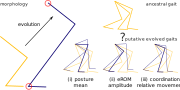
\includegraphics[width=16cm]{./figures/Transferability_Evolution.pdf}
\caption{\label{fig:transferability}\textbf{FCAS facilitates transferability of kinematic data.} A hypothetical, non-isometric evolution of morphology must be compensated by changes in (i) posture, (ii) effective range of motion, and (iii) coordination. By separating these effects in kinematic measurements, evolutionary hypotheses can be tested, and the transfer of coordination patterns from one species to another is improved.}
\end{figure}
\end{change}


Explanatory or even predictive considerations require returning to the construct level, and for legged terrestrial locomotion this would be the level of the joints, e.g. measuring the (joint) angles between segments.
Yet there is a standing problem with that construct: joint angles are constrained by morphology, which has been associated with issues of transferability \citep{Gatesy2011}.
This complicates comparison of joint angles between morphologically disparate groups (e.g. between species, or birth weight categories).
For example, \citet{Gatesy2011} assess that motion transfer between a human and flamingo fails\footnote{\textit{Cf.} \url{https://www.youtube.com/watch?v=1Wh8d9b2Wrw}}, causing ``undesirable motion artifacts'' due to morphological discrepancy\footnote{Another popular example for ``motion transfer'' is the transfer of measured running kinematic data of chicken, \textit{Gallus domesticus}, to animate a \textit{Tyrannosaurus rex}, \textit{cf.} \url{https://www.amnh.org/exhibitions/dinosaurs-ancient-fossils/theropod-biomechanics/walk-dont-run }.}\(^,\)\footnote{These considerations must be flanked by discussions on dynamic similarity \citep{Aerts2023}.}.
They also speculate that underlying patterns of coordination could be invariant to morphological disparity, yet they expose a lack of methods to directly assess coordination.
As shown herein, FCAS enables the isolation of affine components of joint angle profiles, and, by partly removing them, the extraction of measures of coordination.
\chng{I have demonstrated how to generate relative joint angle profiles, which are direct measures of coordination.}
Take a hypothetical lineage which evolves towards elongation \chng{of a single segment} (non-isometric, i.e. the other segments would not elongate similarly; Fig. \ref{fig:transferability}): to retain the ability to walk despite altered morphology, there are three options.
These animals must either (i) change their posture, e.g. by walking with a more extended limb.
In other cases, e.g. an elephant-like, straight limb situation as the ``null'' posture, they must (ii) adjust their effective range of motion to retain locomotor capacity.
Then, (iii) an adjustment of the timing of joint angle changes, i.e. coordination, would follow.
This example re-emphasizes the importance of being able to separate affine components (i, ii) and to process the remaining variables (iii) alone.
The path for future researchers would be to select a suitable phylogenetic branch or example (maybe Tragulidae or Giraffidae, or more broadly Ruminantia), apply FCAS, and measure how a multivariate block of morphological variables correlates to affine and non-affine components of the joint angle data \citep[a suitable method might be Two-Block Partial Least Squares,][]{Rohlf2000}.
FCAS is the door-opener: at first instance, it can help to identify the mismatching aspects which prohibit motion transfer \citep{Gatesy2011}.
It allows for the separation of different logical components of kinematics (especially coordination; Fig. \ref{fig:transferability}), potentially making some of them transferable.
Motion transfer is in fact the extrapolation of kinematic aspects of one species or comparative category to another, i.e. a predictive problem.
The application of a predictive model of NBW kinematics to LBW in this thesis is an implicit form of motion transfer: which age/size would we assign to an NBW which walked like the LBW we observe?
FCAS thus enables predictive modeling at the construct level of locomotion.

\bigskip
The Fourier-method is not always applicable, but often.
Oscillation, i.e. that a limb configuration changes repetitively over time, is a common scheme in all kinds of locomotor patterns: be it a baboon hindlimb flexing-extending-flexing-extending on a bipedal walk to a water hole \citep{Druelle2021}, or be it an ungulate head-nodding in rhythm with its locomotion \citep{Loscher2016}.
There are multiple reasons for the abundance of oscillation in vertebrate locomotion.
The bone-joint system of vertebrates is well approximated by rigid bodies, which can rotate, but hardly translate with respect to each other.
There are other structural constraints, e.g. elastic elements such as the nuchal ligament which has a crucial role in head nodding.
There is neural organization: brain circuits are known to exhibit oscillations as well \citep{Gupta2016}, which might project downstream.
Furthermore, the evolution-like optimization of behavioral tasks: there is little use to gain efficiency in a one-time control unit, yet repeated modules of a task are worth adjustment; this situation might have favored recurrent locomotor modes (but note that those are not omnipresent: think of cephalopod benthic crawling).
In the many cases which show repetitive or recurrent behavior, Fourier analysis is the natural first choice for transformation.
\section{\chng{Methodological Advances}}
\label{sec:org87de9a6}
\begin{change}
To summarize: the Fourier method presented herein complements existing analysis strategies for locomotor kinematics by transforming the data to the frequency domain.
This enables the isolation of affine components, which quantify the dynamic posture, effective range of motion, and the coordination of segments.
Though these components could in principle be extracted from raw profiles, the transformation yields them directly.
The advantages are the following.
\begin{itemize}
\item The transformation changes the \textbf{data structure}. Fourier coefficients are more accessible to multivariate statistics, such as PCA and statistical modeling (Ch. \ref{cpt:fcas} and \ref{cpt:piglets}).
\item \textbf{Information retention:} FSD conserves information and is reversible, which means that any model interpolations or predictions can be converted back to kinematic data, which enable dynamic simulations (e.g. to test for stability).
\item FCAS enables \textbf{motion transfer within} a sequence of joints: some or all affine components can be transferred to adjacent joints (Ch. \ref{cpt:fcas}), leaving the residual, relative movement, i.e. coordination.
\item The method is \textbf{complementary} with existing analysis strategies: for example, one can revert the ``coordination'' residual of an FCAS to temporal profiles and perform statistical parametric mapping (appendix \ref{cpt:spm1d}).
\item \textbf{Motion transfer among} study groups: because of the separation of affines and the altered data structure, one can study and test evolutionary trajectories (again, via simulation).
\item Fourier Series and its inversion are trivial to apply, they are \textbf{deterministic transformations}, and code is readily available or easy to obtain in any common programming language (Ch. \ref{appendix:code}).
\end{itemize}


These new possibilities come with a major limitation: Fourier Series decomposition demands temporal periodicity.
Joint angle profiles must be cyclic, i.e. end at the angle where they started.
Another limitation is that rather complex profiles might theoretically require a rather high number of coefficients, as do situations with multiple joints and 3D angles (which were not exhaustively explored in this work).

On the other hand, the nature of locomotion is that there are oscillating limb elements which often move in cyclical patterns.
There are non-invasive tricks to achieve cyclicity, some of which I discussed herein (e.g. end-start matching, \ref{properties:endstart}).


This connects the first two parts of this thesis to the third one.
It would have been desirable to link Fourier coefficients of piglet kinematics to dynamic simulations of their limb segments.
For example, an immediate question is which segment movements are responsible for which components of joint moments.
Because of the inconclusive attempts to extract inertial properties from CT scans, and because of the reported inaccuracies in markerless motion tracking, I failed to establish such links between kinematics and dynamics (Ch. \ref{cpt:inertials}).
I anticipate that frequency domain considerations hold some unexplored potential in this direction.


Finally, there is some benefit in using probabilistic frameworks when modeling locomotion.
The motor output of biological systems is intrinsically variable, and an animal which is stable on one stride can tumble on the next one.
Working with likelihoods and probabilities of kinematic patterns seems to better reflect the nature of the process.
\end{change}
\section{How and Why Piglets Move}
\label{sec:orgf94ae68}
The primary goal of this thesis was to falsify the hypothesis that there are differences in locomotion of low- and normal birth weight piglets (LBW and NBW, Ch. \ref{cpt:generalintro}).
There are two main aspects in which the study groups could differ: in kinematics (\emph{how} animal limb segments move) and dynamics (\emph{why} animal limb segments move as observed).
And there are putatively confounding effects: locomotor maturation (i.e. age), size and weight of the animals \citep[i.e. physical appearance, cf.][]{Aerts2023}, and the variability of locomotor behavior.


Previous studies from our group have compared kinematics on the level of spatiotemporal characteristics of newborn piglet gait \citep{VandenHole2018}.
They discussed delayed locomotor maturation as a proximal explanation of the observed difference.
I herein extended their analysis and confirmed maturational delay by training probabilistic models on the FCAS data of a large number of NBW piglet strides, applied to LBW observations (Ch. \ref{cpt:piglets}).
The FCAS data entering the model contains practically all kinematic information which could be used to distinguish the study groups.
The predictive models accurately incorporate the variability of the phenomenon.
The models predict size and weight of the LBW piglets as if they were ``normal'', i.e. there are no apparent kinematic differences which would lead the model to infer non-normal subject characteristics.
\chng{This finding must be taken with the discussed grain of salt: conceptually, indifference is hard to prove with the predictive modeling strategy chosen herein, and of course more data would be desirable to settle the case.}
The only differences found are related to the age of LBW piglets.
This indicates that, if models would not consider age or maturation as a model factor, low- and normal birth weight piglet locomotion would be indistinguishable.
The ``age'' model provided evidence that maturation of LBW locomotion halts approximately four hours \emph{post partum} (developmental delay).
We suspect competition within litters and limited metabolic reserves as the reason for developmental delay \citep{VandenHole2019}.

Note that these observations are restricted to walking gait at voluntary speed; we cannot exclude more obvious LBW/NBW differences emerging in more challenging motor tasks.
However, the apparent developmental delay in even this basic motor skill indicates the high sensitivity of the method.
Also, the relevance of any hypothetical, ``more challenging'' stair, treadmill, or wind tunnel experiment for animals whose major priority is to find and access their mother's teats is questionable.
Overall, the models provide \chng{at least some} evidence against the existence of fundamental differences in \emph{how} LBW and NBW piglets move: their coordination seems innate.



\begin{figure}[p]
\centering
\includegraphics[width=12cm]{./figures/piglet_xromm_t02_0214.png}
\caption{\label{fig:piglet_xromm}\textbf{XROMM using Python and Blender}, unpublished. Full video (\url{https://ody.sh/fZe3OpgHGN}) and code (\url{https://git.sr.ht/\~falk/foss\_xromm}) are available.}
\end{figure}

In fact, this lack of differences in the collective output of the animals neuromotor system is surprising.
The FCAS data quantifies joint angle profiles - \chng{which} are indifferent to size.
Yet piglets of low- and normal birth weight operate under different body mass constraints: NBW are about twice as heavy as LBW.
To produce the same kinematics, one would think that they must tune their motors differently, like using different gears.
These would be differences in \emph{why} we observe the (indistinguishable) movements.
Different weight implies different physical constraints, size does matter \citep{Aerts2023}.

Yet we encountered conceptual and practical issues in addressing this second big question (i.e. \emph{why} they move as observed).
The first issue is a practical one (Ch. \ref{cpt:inertials}): inertial parameters, which others have extracted from calibrated CT scans, cannot be determined at sufficient accuracy.
Then, again, there is the issue of variability, as evident from the study of kinematics (Ch. \ref{cpt:piglets}):
differences between NBW and LBW (when normalized for size) seem to be lower in magnitude than the effect of maturation, and lower than normal variability of the behavior.
This was actually confirmed by analysis of 3D kinematics (which we did, unpublished): we originally attempted the full experimental procedure for XROMM.
Of course those recordings are variable, but of the 392 recordings we obtained in several recording sessions in summer 2019, not a single one showed locomotion which strictly fulfilled the ``steady state'' criterion and gave single limb forces (hitting the force plate correctly was likely, but not guaranteed, and happened in 189 recordings, 85 of them walking gait).
Not a single stride could be considered ``representative'', because young piglets in our setup literally always tumbled, jumped, sidestepped, stopped shortly after, or interfered with each other, both LBW and NBW.
The XROMM and inverse dynamics procedure is a low through-put method, and it was not possible to \chng{track landmarks on} a sufficient number of strides to assess LBW differences in joint moment orchestration on the background of motor variability.


These issues notwithstanding, I succeeded in porting the XROMM workflow \citep{Brainerd2010} to an alternative software environment (cf. \url{https://git.sr.ht/\~falk/foss\_xromm}, Fig. \ref{fig:piglet_xromm}).
This workflow includes the complete calculation of inverse dynamics, i.e. joint forces and moments can be visualized.
The software conventionally used for XROMM caused issues: due to its large dependency tree and lack of documentation, XMALab (Brown University, USA, \url{https://xromm.org}) was dysfunctional on the Linux operating system for about half a year during the course of this project; Maya AudoDesk is non-free software.
Except for ORS Dragonfly (Object Research Systems, Canada, \url{https://www.theobjects.com}), which was used for CT segmentation but could be replaced by 3D Slicer (Slicer Community, \url{https://www.slicer.org}), all the tools in the adapted workflow are free and open source.
The example animation (\url{https://ody.sh/fZe3OpgHGN}) can be viewed in Blender (The Blender Foundation, \url{https://blender.org}) from any perspective, and replayed at self-chosen speed.
At the current (incomplete) stage of development, we observe segment position glitches when markers enter or leave the focal volume of the biplanar x-ray.
Also, joint forces and moments do not seem to withstand a visual quality check (their direction and magnitude are sometimes questionable, which falls within the error margin of inertial properties).
This might be an interesting, publishable observation, or a ``bug''; ultimately an error in the computational pipeline cannot be excluded.
Worth noting is that others are currently working in similar directions to open up software alternatives to the conventional XROMM workflow \citep{Falkingham2023}.
At any rate, the primary issues remain the workload of the low through-put XROMM procedure, in contrast to the high through-put demand of appropriate statistics, given the variability of locomotion, coupled with the inaccuracy in determination of inertial segment properties.

The few (three, non-steady) strides which I analyzed and visualized with XROMM techniques with considerable efforts are not representative and cannot provide falsifying evidence with regard to birth-weight dependent differences in piglet locomotor dynamics.


This of course does not imply that there can be no studies of few, representative behavioral observations.
It must be emphasized once more that this major limitation of the present study is tied to two things: the fact that subjects are newborns, and the research question posed herein.
The high variability in locomotor behavior is a specific feature of the ``newborn piglet'' model; at later ages, locomotor behavior stabilizes and becomes more recurrent.
Our research question was whether one can falsify diagnostic differences in LBW and NBW piglets, and the answer must account for stochastic variation to exclude co-incidental findings.
In many other situations, there is either no reason to assume that measurement uncertainty and variability in a behavior are considerable, or they would not prohibit general mechanistic conclusions \citep[e.g.][]{Aerts1998,Astley2012,Montuelle2015}.
Single or rare observations of a behavior can be instructive in many regards \citep[e.g.][]{Druelle2020,Scheidt2022,Dawson2011,Schwarz2020}.
Thus, with most other study settings and subjects, mechanistic evaluations of single strides or actions can generate valuable insights into the workings of the vertebrate musculoskeletal system.


To summarize: this project provided evidence that there is little difference in \emph{how} LBW and NBW piglets move.
Though differences in \emph{why} segments move in a particular way are unlikely in the light of this first finding, methodological limitations prohibited definitive conclusions on dynamic differences in the study groups.
\section{Piglets, Baboons, and Humans}
\label{sec:orgabf5a34}
An important premise of this project was that piglets are a valid model species for humans, in terms of locomotion.
This premise demands constant revision.


Piglets have long been suggested as a model species for human newborns \citep{Book1974,Cooper1975,Mayerl2023}, though there might be alternatives \citep{Mellor1986}.
This suggestion is perfectly justified in the fact that it can be ethically problematic to study human newborns, especially on individuals burdened with an impeded or altered development trajectory.
Piglets are social, sedentary, and share similarity in their appearance (hairless, rotund habitus).
Of course, one has to carefully discuss differences and similarities with the model species, and evaluate alternatives.

One aspect which sets piglets apart from other mammalian model organisms is the relatively high frequency of occurrence of IUGR, Intra-Uterine Growth Retardation \citep{Widdowson1971,Wu2006,VanGinneken2022}.
This diagnosis is different from low birth weight \citep{Wootton1983}, i.e. the lowest quantile of weights in a litter.
Then there is also preterm birth: preterm individuals can have a weight which is lower than normal, but appropriate for gestational age.
Preterms can have low weight for gestational age, or even IUGR, thus double or triple the issues.
Finally, there is low vitality \citep{VandenHole2018}, which is a momentary performance measure (locomotion/respiration scoring), likely linked to the other three state variables.
The situation is complex, classification non-trivial, and there is persistent debate on which indicators matter in which situation.


Nevertheless, researchers study newborn piglets, tracing back epidemiological or congenital issues to histological or structural anomalies.
These can be neurological studies: piglets are somewhat similar to humans in the way their cerebral cortex develops \citep[e.g.][]{Lind2007}, they are available for gene editing \citep{Lind2007}, and a lot of research has focused on neural development in piglets and implications for human infants \citep{Conrad2012,Radlowski2014,Leyshon2016,Mudd2017,Dickerson1971,Fanous2020}.
The piglet model has enabled progress with regard to the research of respiratory problems \citep{Williams1974,Spengler2019}, metabolic issues \citep{Mellor1986,MotaRojas2011,VandenHole2019}, mastication and gut (un-)health \citep{Che2010,Cilieborg2011,Sangild2006,DInca2011,VandenHole2021,Mayerl2023b}.

Maybe most importantly for this thesis, muscle and bone histology and function have been studied \citep{VandenHole2018b,Alvarenga2013,Andersen2016,Aerts2023,Magrini2023}.
Results vary, indicating differences in locomotor performance and muscle mass, but failing to associate them with differences in fibre composition or force generating capacity.

Yet, common to all the organ systems under investigation, it must be stated that analogies of human infants and piglets are usually related to homogeneities on the cellular- or tissue level.
Whereas developmental anomalies in gut, lung, and brain tissue can be related to dysfunctions in neonates of both species, characteristic anomalies of muscle tissue are lacking.
Therefore, though it seems tempting to turn to piglets in light of all the prior research, it might be questionable to choose them as a model \emph{for musculoskeletal aspects}, or even for behavioral aspects which rely on that system.


Other characteristics of the piglet prohibit transfer of findings to our own species, with regard to locomotion.
They are rather precocial \citep{Wischner2009,JYoung2023}, and locomotion of newborns matures at a baffling pace \citep{VandenHole2017,VandenHole2018}.
They are unguligrade, quadrupedal, strictly non-arboreal, and it must be assumed that during the approximately 94 million years of evolution that separate us \citep{Timetree2017} their neural and musculoskeletal anatomy and morphology adapted to different locomotor constraints.


To conclude, I must re-emphasize that piglets are an appropriate and inevitable model species with regard to anomalies on various organ systems.
However, there is little reason to expect relevant conclusions about human locomotor development from piglet research: our locomotor systems are fundamentally different.
Additionally, I quantified a lack of differences in locomotion between low- and normal birth weight piglets (Ch. \ref{cpt:piglets}): it must be assumed that motor control in precocial animals is innate and therefore locomotor capacity indistinguishable.
I cannot exclude that the most severe IUGR or preterm conditions can elicit deficits in kinematics, tracing to impeded neural or musculoskeletal development.
Also, metabolic difference are likely, limiting endurance and vitality of LBWs, which I did not quantify.
But even if such differences occur, they cannot be easily extrapolated to humans.


This opens the discussion about alternative model species.
Non-human primates, e.g. baboons, are sufficiently similar to humans in anatomy and habitus, and their usefulness in medical and evolutionary research is widely accepted \citep{Nardone2017,Liang2023,Aerts2023b,Druelle2021,BoulinguezAmbroise2021}.
Their developmental trajectory is less steep than that of piglets (Ch. \ref{cpt:statistics}), but still on a manageable timescale for longitudinal studies \citep{Druelle2017}.
Ethical concerns in using primates might weigh more strongly (for reasons unknown).
Those objections can be partially mitigated for the kind of locomotor research demonstrated herein:
kinematic studies from calibrated videography are non-invasive.
The inaccuracies of inertial measurements (Ch. \ref{cpt:inertials}) justify doubt on the common practice of euthanizing individuals after experiments; one could as well use naturally deceased specimens, model data, or literature data to transfer the measured inertials to new observations (which would also enable longitudinal inverse dynamic studies).
All this of course demands ethical assessment of, amongst more, proportionate radiation dose (especially on young individuals), appropriate experimental circumstances (e.g. habituation requirement), and general welfare \citep{Young2018}.
The main limiting factor for such studies is the availability of non-human primates and their offspring, even more of IUGR-like conditions, which, as is often argued, is one of the benefits of using domestic piglets as a model.

Yet in the light of the present thesis, it seems more worthwhile to strive for appropriate conditions and experimental circumstances to study species which are more closely related to humans.


\clearpage
\section{Conclusion}
\label{sec:org4656fa9}
Independent of the choice of model species, this thesis presented a number of advances in developmental or general studies of locomotor behavior.

\bigskip
Conventional studies of kinematics mainly rely on irreversibly derived spatiotemporal variables.

Raw kinematic traces are often qualitatively compared, yet inaccessible for multivariate statistical analysis.
Fourier Analysis methods are known and rarely used, yet a subtle completion made them more accessible for kinematic analysis: equation \eqref{eqn:affines_phase}, which determines the main phase of a signal.
Together with the delay theorem, a cyclic joint angle profile can be ``rolled'' around the stride cycle for precise temporal alignment.
The affine components (mean, amplitude, phase) of the joint angle profiles can be isolated, allowing a Procrustes-like alignment and more relevant quantitative comparison of temporal patterns in joint angle movement.

I have demonstrated the potential of this set of mathematical tricks on a broad data set of ungulates (comparative/descriptive) and on a longitudinal, developmental data set from piglet kinematics (comparative/predictive).


\bigskip
Transforming kinematic data to the frequency domain and extracting affine components opens up countless possibilities for data analysis.

Variability in locomotor output might be considered a nuisance, yet especially in neonates, variability and the progressive reduction of it are arguably a feature of the system.
Variability enables learning and locomotor maturation; even seemingly innate neuromotor control has to pass the ``reality test''.
Being able to quantify and compare this feature is a huge advantage of probabilistic models.
Predictive modeling, in particular, can be implemented to compare groups (as demonstrated), refine model design, support hypothesis building; models can take an evolutionary, comparative, longitudinal or cross-sectional, or exploratory flavor, or many more.
The modeling toolbox chosen herein has proven to be sufficiently adaptable to handle even complex model constructs, which relate subject characteristics (including morphometrics), spatiotemporal variables, and raw kinematics in FCAS form.
The achievement of the author with regard to probabilistic modeling is mainly educational: these methods are popular in other fields, yet I daresay that few biomechanists are fully aware of their potential.
Consequently, all code produced for this thesis is publicly available for others to adapt and replicate.

With all these data types and modeling capabilities at hand, future researchers can fine tune their models to answer highly specific questions about study subjects and their locomotor development.


\bigskip
In contrast to kinematic data analysis and modeling, my contribution to inverse dynamic modeling is less than what I hoped to achieve.

As discussed above, this is due to the discrepancy in data throughput of the inverse dynamic workflow, and variability of the phenomenon of interest.
Also, initial technical misconceptions about CT scans (Ch. \ref{cpt:inertials}) have temporarily misled my efforts; there were visible problems in the outcome of my custom-made inverse dynamics workflow.
In reaction, the ``flying femur'' experiment as a reductive approach enabled the understanding of all details of the workflow.
This included a sensitivity analysis, which reveals surprisingly high error margins for the inertial properties, which might be prohibitive for inverse dynamic calculations.
I take this as a clear reminder that for anything we measure, we should put all necessary efforts into understanding the mechanistic fundamentals of our measurement, and we must keep track of measurement uncertainty.

Both the reductive approach and the sensitivity analysis are advisable strategies hopefully adopted by future biomechanists.

\bigskip
It is my sincere hope that other researchers take these analysis tools, reproduce, adapt, and correct them where needed, and improve our understanding of how and why various animals move in different phases and circumstances of their existence.
I hope this goal explains some extensive, tutorial-like chapters within this thesis, and it hopefully excuses the colloquial tone of some paragraphs which might not have been to the intended entertainment or taste of every recipient.
\bigskip


Thank you for your interest in my work!
